\documentclass[../thesis.tex]{subfiles}
% Separate preamble for this subfile. This preamble is loaded last, so one can override various functions before \begin{document}

% Better comment extension for Vscode colors these comments differently
% Normal comment color
% * Important information
% ! ALERT
% ? Question
% TODO stuff to do
% // This is strikethrough


\begin{document}
%
%
%\begin{remark}
%    Nevertheless, by arranging unit cubes into a \emph{new} tile, one can get an aperiodic tiling for all $d\geq3$, as done in \cite{lagariasKellerCubetilingConjecture1992}. (Max: Given that it is actually true that this organization/new tile/ of unit cubes EXCLUSIVELY tiles non-periodically. Not known to me yet). The fact that the new tile only consists of unit cubes in a particular arrangement is not equivalent to the statement that there \emph{are} aperiodic cube tilings in all $d\geq3$ as stated in \cite{lagariasOrthonormalBasesExponentials2000,liuUniformityNonUniformGabor2003}, as one considers a tiling which, in fact, is \textsc{not} a cube, only consisting of cubes; and by the very definition of aperiodicity means that it must exclusively tile non-periodically, which \emph{cube tilings} intrinsically do not as highlighted above. Furthermore, \cite{lagariasOrthonormalBasesExponentials2000} provides no source for this "well-known" statement, and \cite{liuUniformityNonUniformGabor2003} makes a reference to \cite{lagariasKellerCubetilingConjecture1992}, but the explanation here is both insufficient and unclear, as this result is \textsc{never} stated anywhere. (Max: If I am wrong with this, then I cannot read. This can very well be the case when it comes to math, but I am pretty certain of this latter sentence. It can be true that the result is implied by the paper or somehow obvious in a way I cannot understand, but that is not a clear and sufficient statement of the result from my undergraduate perspective.)
%\end{remark}

APERIODIC: $\mathbf{T}_\tau: \widetilde{\Lambda} \rightarrow \widetilde{\Lambda}'$, if $\widetilde{\Lambda}' = \widetilde{\Lambda}$ then the translation is invariant ? 
or for a more general tiling set $\mathbf{T}_\tau: \Lambda \rightarrow \Lambda'$, if $\Lambda = \Lambda'$ then the translation is invariant.


\SigridChange{Intro optinons:}

In this section, we will show the following result. 
\SigridComment{ or }

The topic for this \namecref{sec:aperi_cube} is a "new" result first put forward by Lagarias (, Reeds, and Wang??) in \cite{lagariasOrthonormalBasesExponentials2000}, however no proof or reference to the literature was attached \SigridChange{(needs rephrasing!)}. The statement has later been referenced in \cite{liuUniformityNonUniformGabor2003}, although with incorrect reference. After correspondence with Lagarias himself, the main result of this \namecref{sec:aperi_cube} was submitted as a problem for the American Math Monthly. 

\SigridComment{not sure how to intro this, or whether to put this info in a footnote, or close the section with this.}

Correct citation?
\cite{haugeTitle}

\begin{theorem}
    There exists a translational tiling of unit cubes $I^d + \lambda$ in $\R^d$ for $\lambda\in \Lambda$ in all dimensions $d\geq3$, in which the tiling set $\Lambda$ constitutes an aperiodic tiling. 
\end{theorem}

For convenience, we will label unit cubes in the tiling by their corner coordinates which will be given by the vector $x = \brac{x_1,\dots,x_d} \in \R^d$. Note that it is essential that all unit cubes are labeled using the same corner; otherwise, the notation we will employ will lead to overlap. Furthermore, we will denote a unit cube that is parallel to an axis by
\begin{equation*}
    \mathcal{C}\bracMed{x_1,\dots,x_d} = \braqMed{(x_1,\dots,x_d) + (t_1,\dots,t_d) : 0 \leq t_j \leq 1}
\end{equation*} 
where $x\in \R^d$ is the specified corner coordinate. We say that this is an \emph{axis-paralell unit cube}. 

The proof will provide a specific way to construct an aperiodic tiling of unit cubes in any dimension from a fully periodic tiling of unit cubes $\Lambda$ in $\R^d$. We will initially consider a lattice tiling of unit cubes such that all cube-corners will be in an integer lattice, meaning $\Lambda = \Z^d$. Using the following translation, we create the new tiling denoted by $\widetilde{\Lambda}$, which we will show is aperiodic. The translation consists of shifting exactly two specific disjoint columns of unit cubes and leaving the remaining unit cubes in the $\Z^d$-tiling in place. The underlying idea is that the shifted columns create dislocations in the fully periodic tiling of unit cubes $\Lambda$. We can think of these dislocations as line or skew-line defects. The critical observation is that the position of the defects can be detected locally and that these positions move when $\widetilde{\Lambda}$ undergoes a translation. Since translated tilings of $\widetilde{\Lambda}$ will differ from the original tiling $\widetilde{\Lambda}$, we have that $\widetilde{\Lambda}$ will have no non-trivial translation symmetry, and hence must necessarily be aperiodic. 

\begin{remark}
    The use of \emph{column} in this \namecref{sec:aperi_cube} differs from how the term has been used in the rest of the thesis. Here, a column is considered to be a one-dimensional column of unit cubes in one of the $d$ coordinate directions. As an example, for $d=2$, what we previously denoted as a row or a column of unit cubes is now considered a column of unit cubes in either the first or second coordinate direction, respectively. \SigridComment{write something on why? We make this distinction as in higher coordinates$\dots$} 
\end{remark}

\SigridChangeTwo{Begin proof environment here?}

Before generalizing it to higher dimensions, we prove the result for dimension $d=3$. Here we displace two columns of unit cubes with corner coordinates 
\begin{align*}
    \bracMed{m_1,0,1},& \quad m_1 \in \Z,\\
    \bracMed{0,1,m_3},& \quad m_3 \in \Z,
\end{align*}
shifting each of them with the respective translation vectors $\upsilon' = \brac{\frac{1}{2},0,0}$ and $\upsilon'' = \brac{0,0,\frac{1}{2}}$ so that
\begin{align*}
    \bracMed{m_1,0,1} \xlongrightarrow[]{\upsilon'} \bracMed{m_1 + \frac{1}{2} ,0,1}, \quad  &\text{ for all } m_1 \in \Z,\\
    \bracMed{0,1,m_3} \xlongrightarrow[]{\upsilon''} \bracMed{0,1,m_3 + \frac{1}{2} },    \quad  &\text{ for all }  m_3 \in \Z.
\end{align*}
Observe that the column of unit cubes covers exactly the same set after the translation since the translation is in the same direction as the column itself 
\begin{align*}
    \braqMed{ \bracMed{x_1, 0+t_2,1+t_3} : 0 \leq t_j \leq 1, x_1\in\R} \xlongrightarrow[]{\upsilon'} & \braqMed{ \bracMed{x_1, 0+t_2,1+t_3} : 0 \leq t_j \leq 1, x_1\in\R},\\
    \braqMed{ \bracMed{0+t_1,1+t_2,x_3} : 0 \leq t_j \leq 1, x_3\in\R} \xlongrightarrow[]{\upsilon''} & \braqMed{ \bracMed{0+t_1,1+t_2,x_3} : 0 \leq t_j \leq 1, x_3\in\R}.
\end{align*}
In addition, note that both shifted columns are disjoint in $\R^3$ since their middle corner coordinates $x_2$ differ by a non-zero integer. Hence, the new tiling $\widetilde{\Lambda}$ is still a cube-tiling of $\R^3$. To show that $\widetilde{\Lambda}$ is an aperiodic tiling, consider the following. Let $\tau=\brac{\tau_1,\tau_2,\tau_3}\in \R^3$ be a vector which we associate with the translation
\begin{equation*}
    \mathbf{T}_\tau \bracMed{x} = x+\tau = \bracMed{x_1+\tau_1, x_2+\tau_2, x_3+\tau_3},
\end{equation*}
where $x\in \R^3$ is the point on which the translation acts. If the translation maps cube-corners to cube-corners, then the tiling will be invariant under $\mathbf{T}_\tau$. We now show that $\tau=\brac{0,0,0}$ is the only vector that preserves cube-corners and makes $\mathbf{T}_\tau$ invariant \SigridChange{(map?)}. 

We first show that the translation vector $\tau \in \Z^3$. Consider a $2\times 2\times 2$ block of $8$ unit cubes in $\widetilde{\Lambda}$, which do not intersect any part of our translated columns. Note that all unit cubes in our block have integer coordinates. When translating the block, its image under the translation must also be a $2\times 2\times 2$ block of $8$ unit cubes in $\widetilde{\Lambda}$. Since our shifted columns are disjoint, there will be at most $4$ unit cubes from our shifted columns, while the remaining unit cubes must still have integer coordinates. As such, $\tau$ maps an integer vector to another integer vector. That is, $\tau$ maps some cube-corner from the initial block to a cube-corner in the image block, which has an integer corner vector. Hence, $\tau \in \Z^3$. 

Secondly and last, we show that the translation vector $\tau = \brac{0,0,0}$. We first claim that $\tau$ must map each of the two shifted columns into itself. Before proving the claim, we show how the result follows. Therefore, assume the claim is valid. Observe that the translation which maps the first shifted column of unit cubes to itself is one with a translation in the same direction as the shift. That is, we must have $\tau' = (\tau'_1,0,0)$ for any $\tau'_1\in \Z$ since
\begin{equation*}
    \bracMed{m_1 + \frac{1}{2} ,0,1} \xlongrightarrow[]{\tau'} \bracMed{m_1+\tau'_1 + \frac{1}{2} ,0,1}, \quad \text{ for all } m_1 \in \Z,\\
\end{equation*}
which is still the same column of unit cubes as $m_1+\tau'_1\in\Z$. Similarly, for the second shifted column, we must have $\tau'' = (0,0,\tau''_3)$ for any $\tau''_3\in \Z$ since 
\begin{equation*}
    \bracMed{0,1,m_3 + \frac{1}{2} } \xlongrightarrow[]{\tau''} \bracMed{0,1,m_3+\tau''_3 + \frac{1}{2} } , \quad \text{ for all } m_3 \in \Z,\\
\end{equation*}
which is still the same column of unit cubes as $m_3+\tau''_3\in\Z$. To satisfy both translations described by $\tau'$ and $\tau''$ at the same time we must have, $\tau_1 = 0$ from $\tau''$, and $\tau_3 = 0$ from $\tau'$. Last, since $\tau_2'=\tau_2'' = 0$ we have $\tau_2=0$. Hence $\tau = \brac{0,0,0}$.

To show the claim, note that since $\tau\in\Z$, it will, for each cube-corner vector, preserve both; the shifted part, or in this case, the fractional part of a coordinate and also its position in the cube-corner vector. As it is only the two shifted columns that have non-zero fractional parts in the tiling $\widetilde{\Lambda}$, we have that the fractional part will always be in the first coordinate position for the first column, and always the third coordinate position for the second column. Using that $\tau\in\Z$ means that if our initial tiling vector $\tilde{\lambda} \in \widetilde{\Lambda}$ has a non-zero fractional part in some coordinate position, then the image vector of $\tilde{\lambda}$ will have an equal non-zero fractional part in the same coordinate position. The converse is also true. 

To show the $n$-dimensional case, we modify the above arguments. Take the two columns of unit cubes in the initial $\Z^d$-tiling to be the ones with corner coordinates
\begin{align*}
    \bracMed{m_1,1,0, \dots,0}, & \quad m_1 \in \Z,\\
    \bracMed{0,\dots,0,1,m_d},& \quad m_d \in \Z,
\end{align*}
and using a similar shift of $\upsilon' = \brac{\frac{1}{2},0,\dots,0}$ and $\upsilon'' = \brac{0,\dots,0,\frac{1}{2}}$ to get
\begin{align*}
    \bracMed{m_1,1,0, \dots,0} \xlongrightarrow[]{\upsilon'} \bracMed{m_1+\frac{1}{2}, 1, 0, \dots, 0}, \quad  &\text{ for all } m_1 \in \Z,\\
    \bracMed{0,\dots,0,1,m_d} \xlongrightarrow[]{\upsilon''} \bracMed{0, \dots, 0, 1, m_d+\frac{1}{2}},    \quad  &\text{ for all }  m_3 \in \Z.
\end{align*}
Then, using the exact same arguments, but now with a $\overbrace{2\times \dots \times 2}^{d-\text{times}}$ cube, and that the only column preserving translations $\tau'$ and $\tau''$ must be
\begin{align*}
    \tau' =& \bracMed{\tau'_1,0,\dots,0 }, \quad \tau'_1 \in \Z,\\
    \tau'' =& \bracMed{0,\dots,0,\tau''_d}, \quad \tau''_d \in \Z,
\end{align*}
shows that the translation vector $\tau=\brac{0,\dots,0}$ is the zero-vector.


$\square$


\SigridComment{some alternative ending}
Hence we can state the following result using the above as proof

\begin{theorem}
    There exists a translational tiling of unit cubes $I^d + \lambda$ in $\R^d$ for $\lambda\in \Lambda$ in all dimensions $d\geq3$, in which the tiling set $\Lambda$ constitutes an aperiodic tiling. 
\end{theorem}

\begin{figure*}[h!]
    \centering
    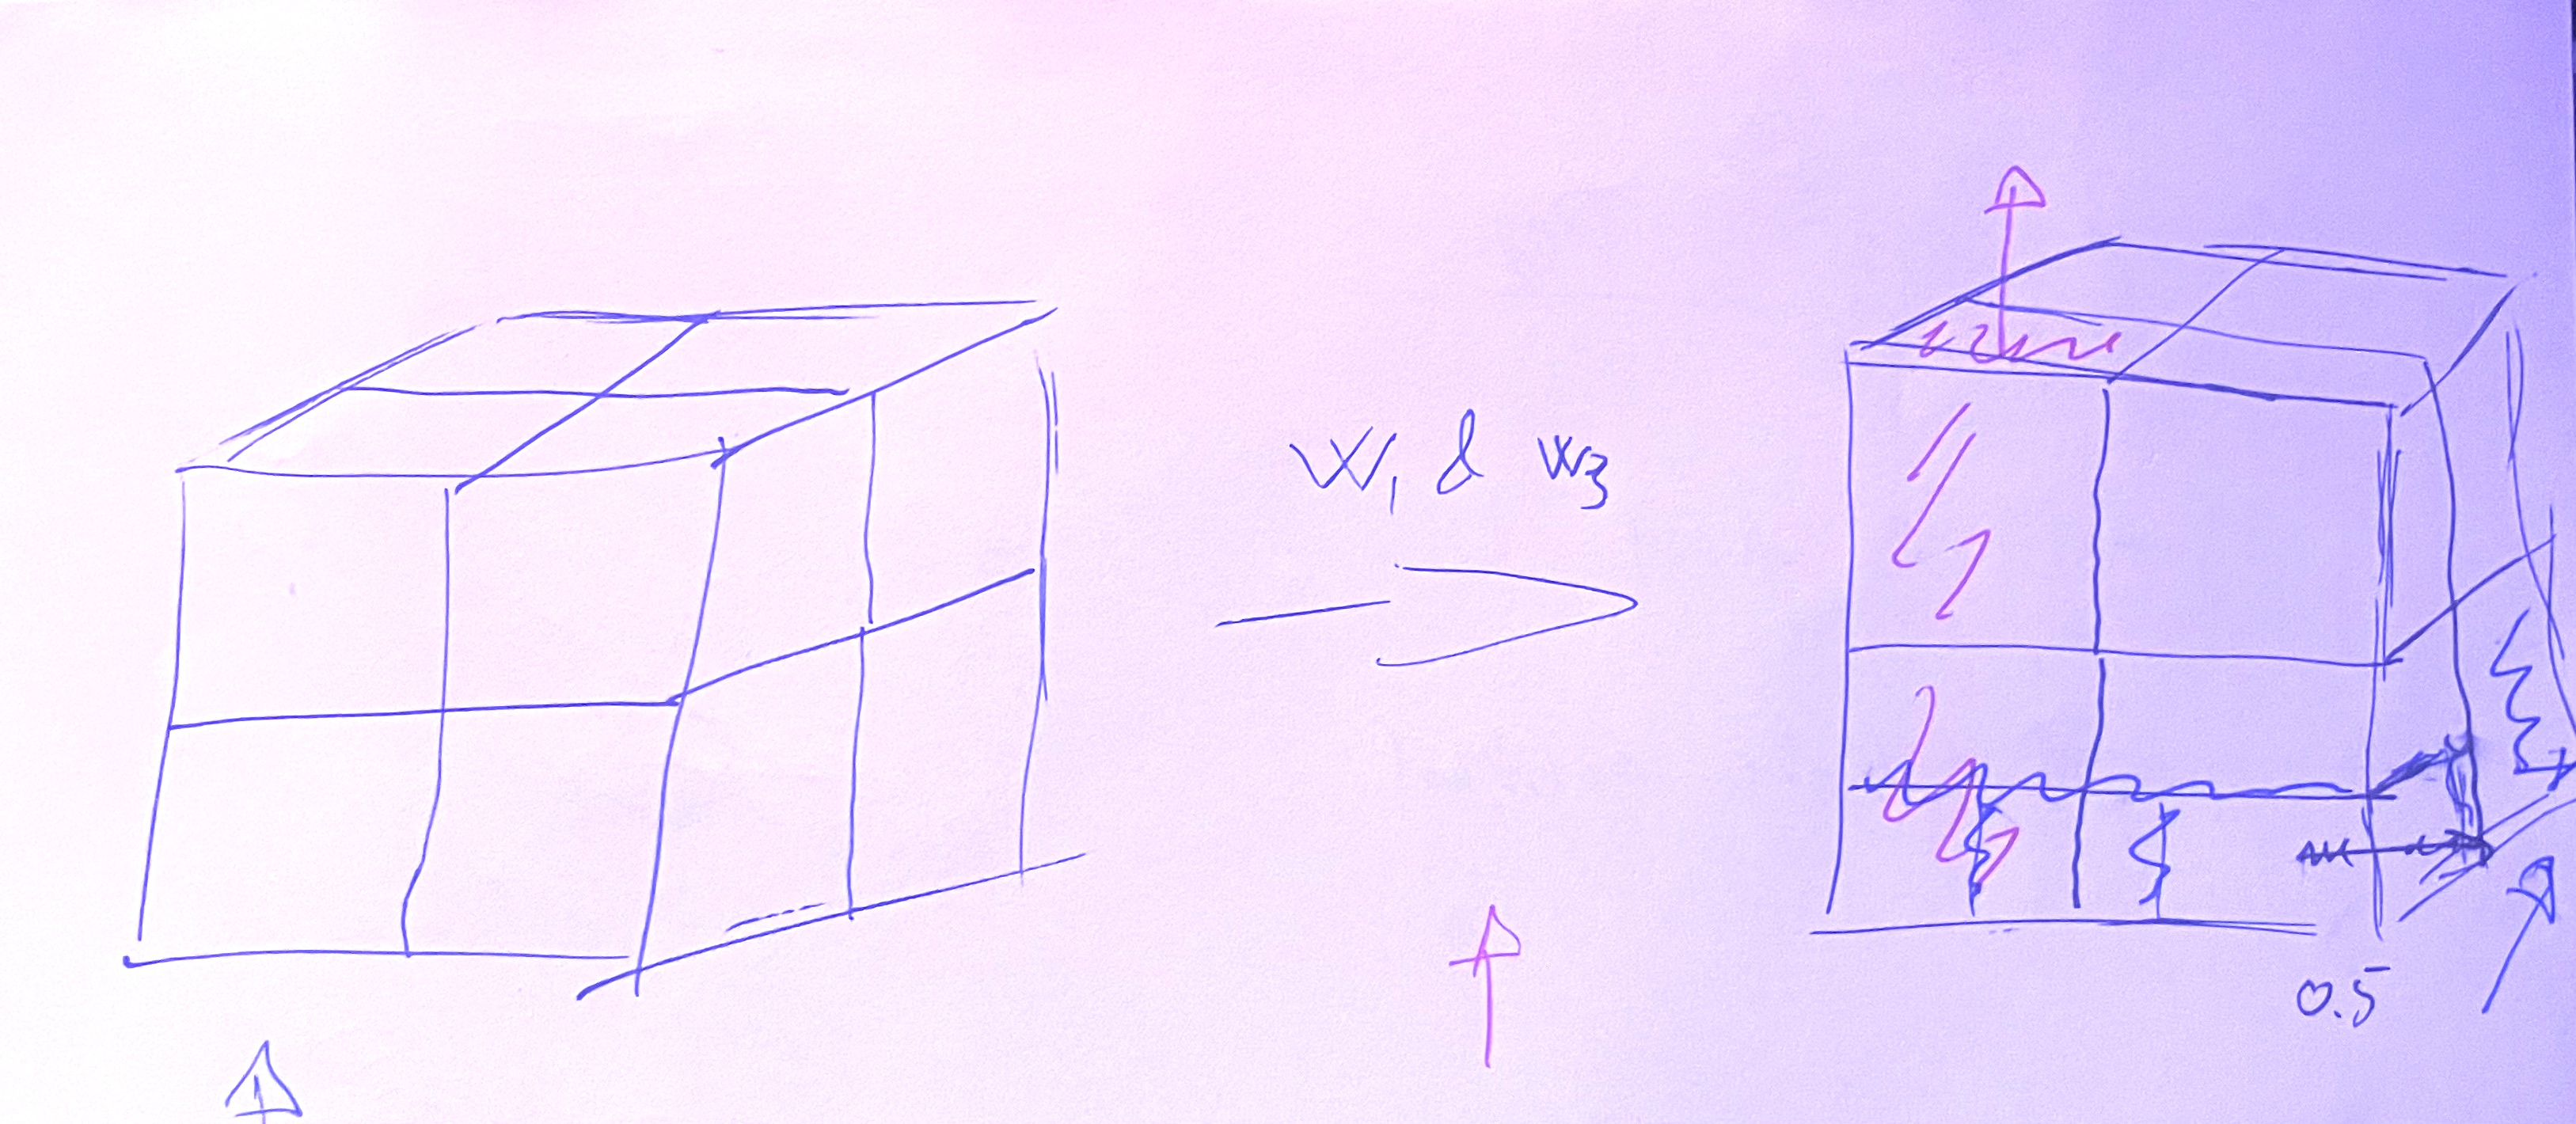
\includegraphics[width=0.87\linewidth]{aper_yeye.jpg}
    \caption{TEXTTEXT lorum blabla, figure placement somewhere nice}
    \label{fig:aperi_cube}
\end{figure*}

Illustrated in FIG:A is the initial lattice tiling $\Lambda$, and illustrated in FIG:B is the constructed aperiodic tiling $\widetilde{\Lambda}$ after translation of $\upsilon'$ and $\upsilon''$. The latter figure also shows that there can be no more than four unit cubes from the shifted columns in a $2\times 2\times 2$ block of cubes. 

\end{document}